\begin{figure}
\centering

\tikzsetnextfilename{cpexamples}

\begin{subfigure}[b]{1\columnwidth}
\centering
% \cfbox{box-gray}{
\resizebox{!}{12mm}{
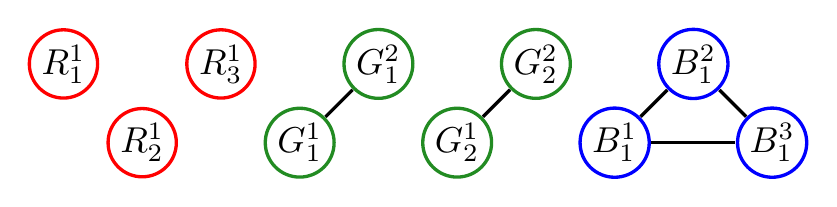
\begin{tikzpicture}[
mynode/.style={draw, circle, very thick, inner sep=1pt, scale=1.3},
myline/.style={draw, very thick},
]

\node[mynode,draw=red] (1) at (-2,-0) {$\xcolor{R}_1^1$};
\node[mynode,draw=red] (2) at (-1,-1) {$\xcolor{R}_2^1$};
\node[mynode,draw=red] (3) at (0,0) {$\xcolor{R}_3^1$};
\node[mynode,draw=ForestGreen] (4) at (1,-1) {$\xcolor{G}_1^1$};
\node[mynode,draw=ForestGreen] (5) at (2,0) {$\xcolor{G}_1^2$};
\node[mynode,draw=ForestGreen] (6) at (3,-1) {$\xcolor{G}_2^1$};
\node[mynode,draw=ForestGreen] (7) at (4,0) {$\xcolor{G}_2^2$};
\node[mynode,draw=blue] (8) at (5,-1) {$\xcolor{B}_1^1$};
\node[mynode,draw=blue] (9) at (6,0) {$\xcolor{B}_1^2$};
\node[mynode,draw=blue] (10) at (7,-1) {$\xcolor{B}_1^3$};

\draw [myline] (4) -- (5);
\draw [myline] (6) -- (7);
\draw [myline] (8) -- (9);
\draw [myline] (8) -- (10);
\draw [myline] (9) -- (10);

\end{tikzpicture}
}
% } 
\caption{\nameref{sec:ch2:example1}. \label{fig:ch2:cpexamples:1}}
\end{subfigure}

\begin{subfigure}[b]{1\columnwidth}
\centering
% \cfbox{box-gray}{
\resizebox{!}{12mm}{
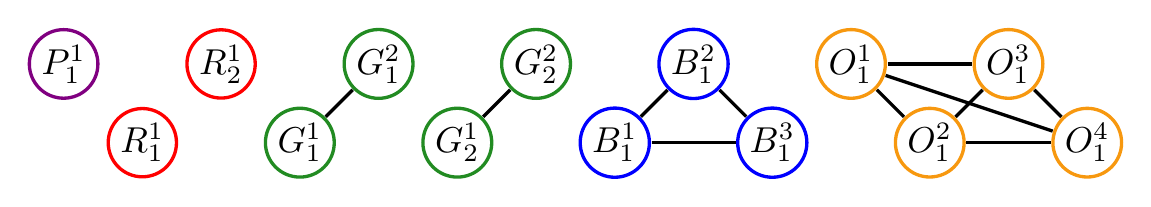
\begin{tikzpicture}[
mynode/.style={draw, circle, very thick, inner sep=1pt, scale=1.3},
myline/.style={draw, very thick},
]

\node[mynode,draw=Purple] (1) at (-2,0) {$\xcolor{P}_1^1$};
\node[mynode,draw=red] (2) at (-1,-1) {$\xcolor{R}_1^1$};
\node[mynode,draw=red] (3) at (0,0) {$\xcolor{R}_2^1$};
\node[mynode,draw=ForestGreen] (4) at (1,-1) {$\xcolor{G}_1^1$};
\node[mynode,draw=ForestGreen] (5) at (2,0) {$\xcolor{G}_1^2$};
\node[mynode,draw=ForestGreen] (6) at (3,-1) {$\xcolor{G}_2^1$};
\node[mynode,draw=ForestGreen] (7) at (4,0) {$\xcolor{G}_2^2$};
\node[mynode,draw=blue] (8) at (5,-1) {$\xcolor{B}_1^1$};
\node[mynode,draw=blue] (9) at (6,0) {$\xcolor{B}_1^2$};
\node[mynode,draw=blue] (10) at (7,-1) {$\xcolor{B}_1^3$};
\node[mynode,draw=YellowOrange] (11) at (8,0) {$\xcolor{O}_1^1$};
\node[mynode,draw=YellowOrange] (12) at (9,-1) {$\xcolor{O}_1^2$};
\node[mynode,draw=YellowOrange] (13) at (10,0) {$\xcolor{O}_1^3$};
\node[mynode,draw=YellowOrange] (14) at (11,-1) {$\xcolor{O}_1^4$};

\draw [myline] (4) -- (5);
\draw [myline] (6) -- (7);
\draw [myline] (8) -- (9);
\draw [myline] (8) -- (10);
\draw [myline] (9) -- (10);
\draw [myline] (11) -- (12);
\draw [myline] (11) -- (13);
\draw [myline] (12) -- (13);
\draw [myline] (11) -- (14);
\draw [myline] (12) -- (14);
\draw [myline] (13) -- (14);

\end{tikzpicture}
}
% }
\caption{\nameref{sec:ch2:example2}. \label{fig:ch2:cpexamples:2}}
\end{subfigure}

\caption{$G^{P}$ graphs for two examples. \label{fig:cpexamples}}

\end{figure}

